\documentclass[tikz,border=2mm]{standalone}
\usetikzlibrary{arrows.meta}

\begin{document}
\begin{tikzpicture}
\foreach \arrowtipkind[count=\i from 0] in {
Circle,
Diamond,
Ellipse,
Kite,
Latex,
Rectangle,
Square,
Stealth,
Triangle,
Turned Square,
Arc Barb,
Bracket,
Hooks,
Tee Barb,
Parenthesis,
Implies,
Butt Cap,
Fast Round,
Fast Triangle,
Round Cap,
Triangle Cap}{\foreach \specs[count=\j from 0] in {round, open, fill=red, {round, fill=blue, length=2.5mm, slant=.5}}{\draw[-{\arrowtipkind[\specs]}, yshift=-1.5*\i cm -0.2*\j cm] (0,0) -- +(1,0)\ifnum\j=0 node[above,midway,font=\scriptsize\ttfamily]{\arrowtipkind}\fi;};};
%%% Tips with particular options:
% Arc Barb[sep, arc=<angle>, length=<dim>, line width=<dim>, width=<dim>, reversed, round, slant=<num>, harpoon, left, right, <color>]
% Bracket[sep, reversed, round, slant=<num>, left, right, harpoon, reversed, <color>]
% Hooks[sep, arc=<angle>, length=<dim>, line width=<dim>, width=<dim>, reversed, round, slant=<num>, harpoon, left, right, <color>]
% Tee Barb[sep, inset=<dim>, inset'=<dim> <num>, line width=<dim>, reversed, round, slant=<num>, harpoon, left, right, <color>] thin thick
% Implies[<color>]
\end{tikzpicture}
\end{document}